A user when attempting to connect to a dual-stacked web service prefers
connecting over IPv6. This is because in POSIX systems,
\texttt{getaddrinfo(\ldots)} resolves a service name to a list of endpoints in
an order that prioritizes an IPv6-upgrade path \cite{rfc6724}.  The dictated
order can dramatically reduce the application responsiveness in situations
where IPv6 connectivity is broken. This is because, the attempt to connect
over an IPv4 endpoint will take place only when the IPv6 connection attempt
has timed out, which can be in the order of seconds.

\begin{figure}[t]
\centering
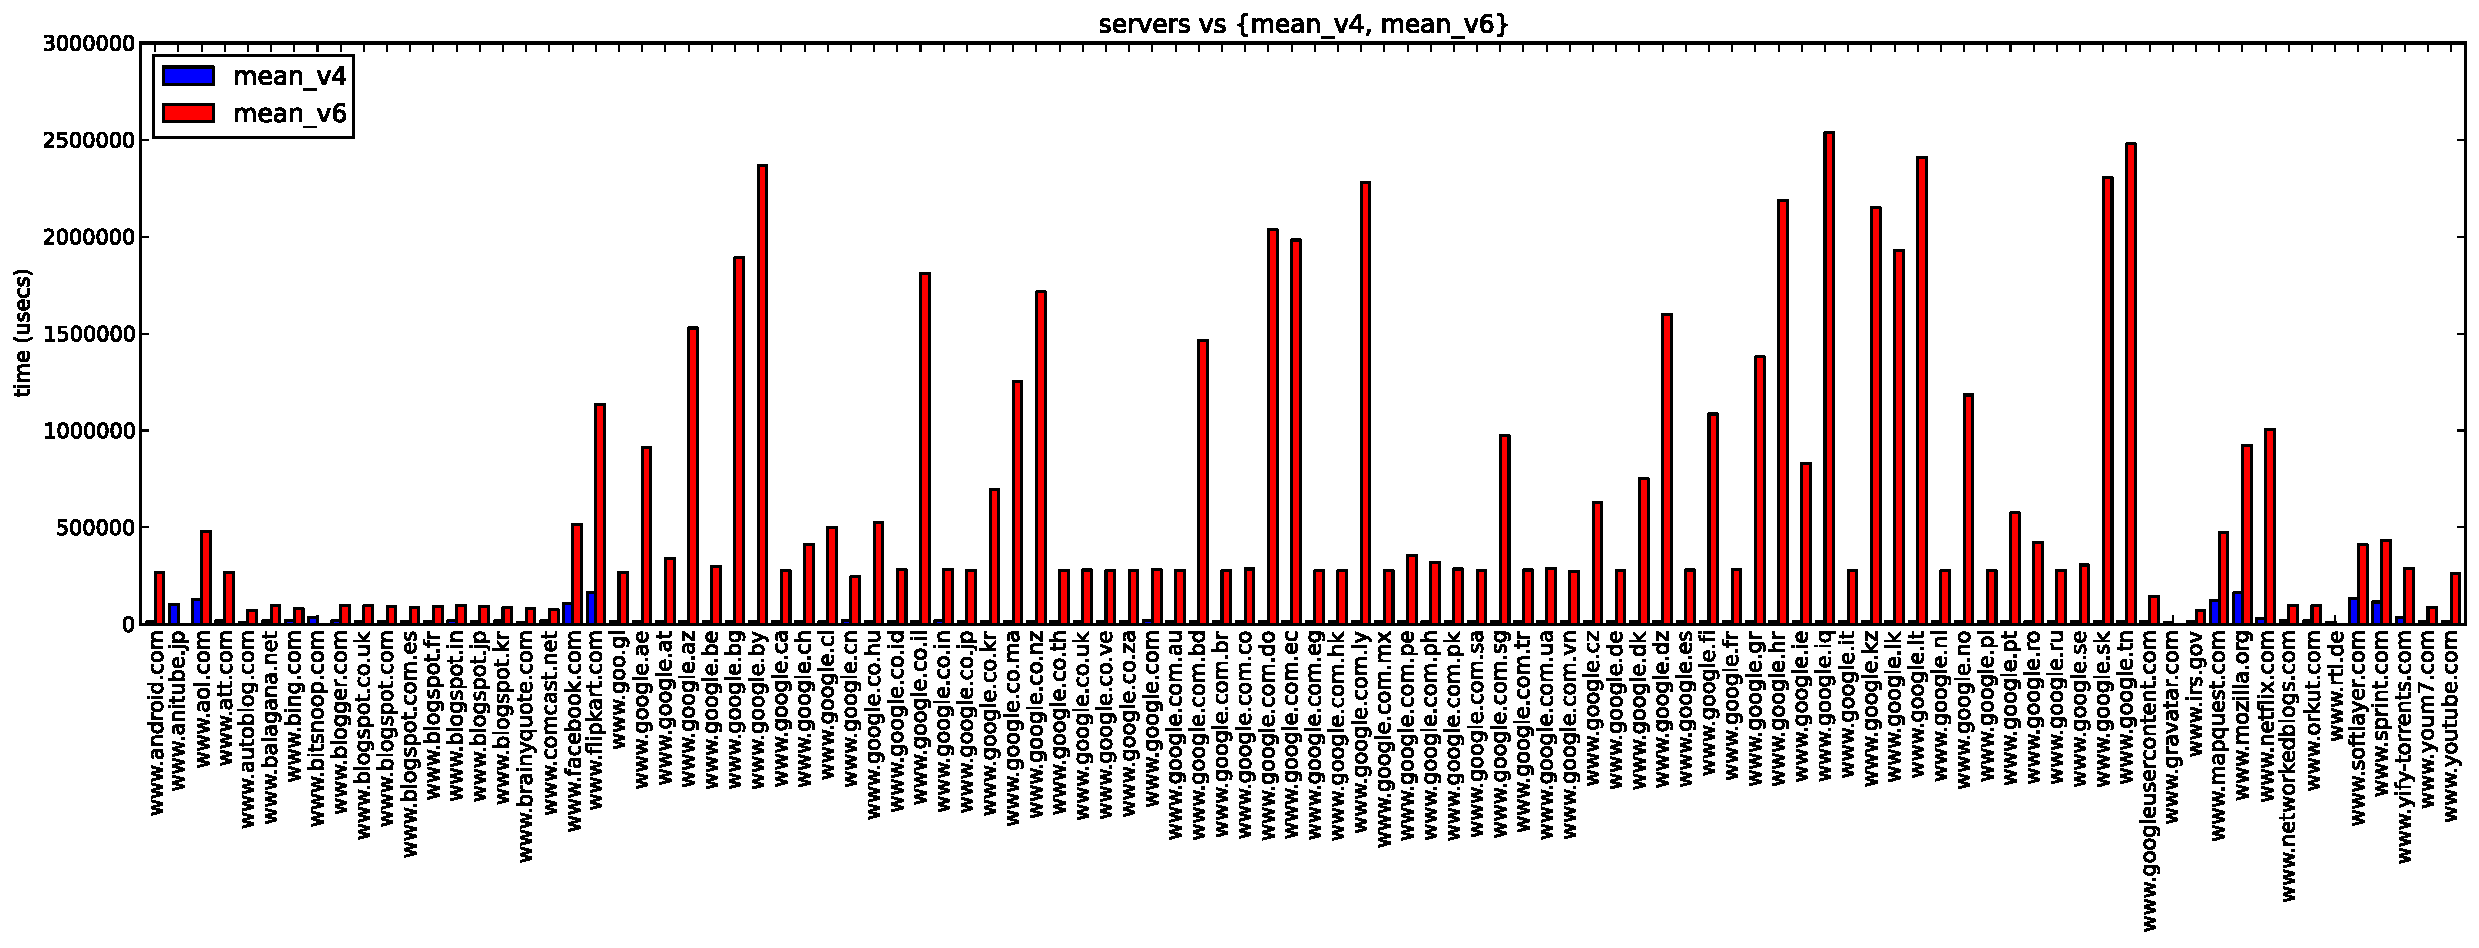
\includegraphics[width=1.0\textwidth]{figures/t28972-mean}
\label{fig:t28972-mean}
\caption{Mean connection times to a list of services. The measurement point is
a virtual machine hosted at greatnet.de. It has IPv4 connectivity via LamdaNet
Communications [AS13237] and IPv6 connectivity via Teredo.}
\end{figure}

%\begin{figure}[h!]
%\centering
%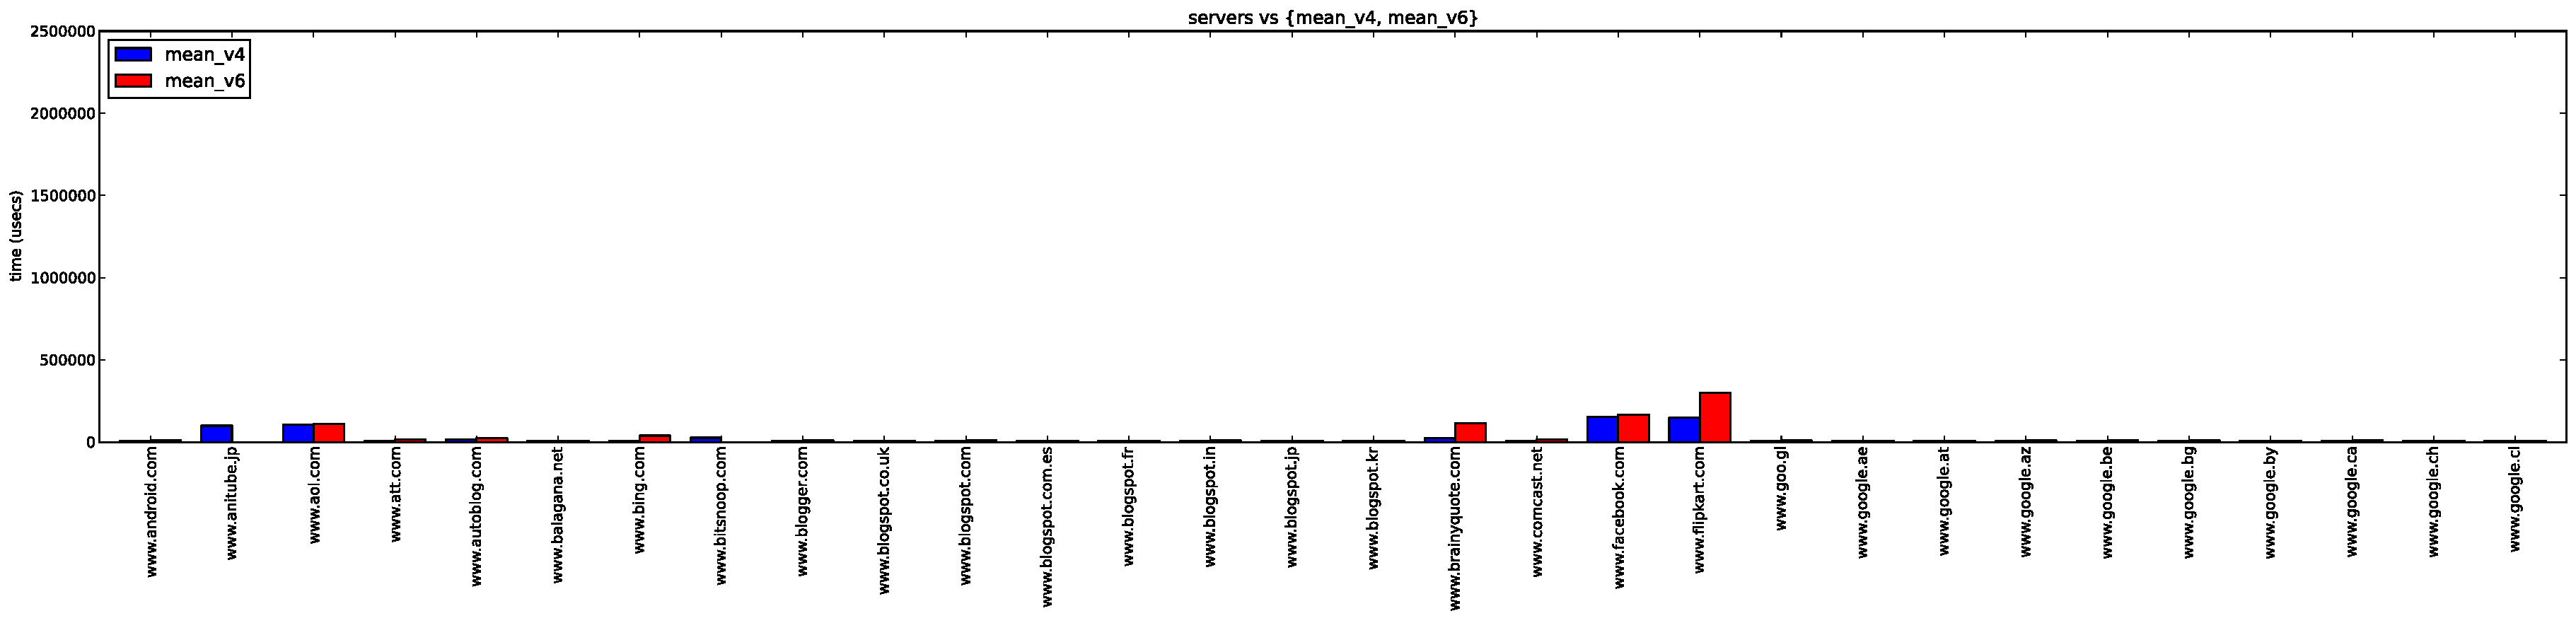
\includegraphics[width=1.0\textwidth]{figures/unimator2-mean}
%\caption{Native IPv4 and Teredo Tunnel}
%\end{figure}

%\begin{figure}[t]
  %\begin{minipage}[t]{0.50\textwidth}
    %\centering
    %\resizebox*{1.0\textwidth}{!}{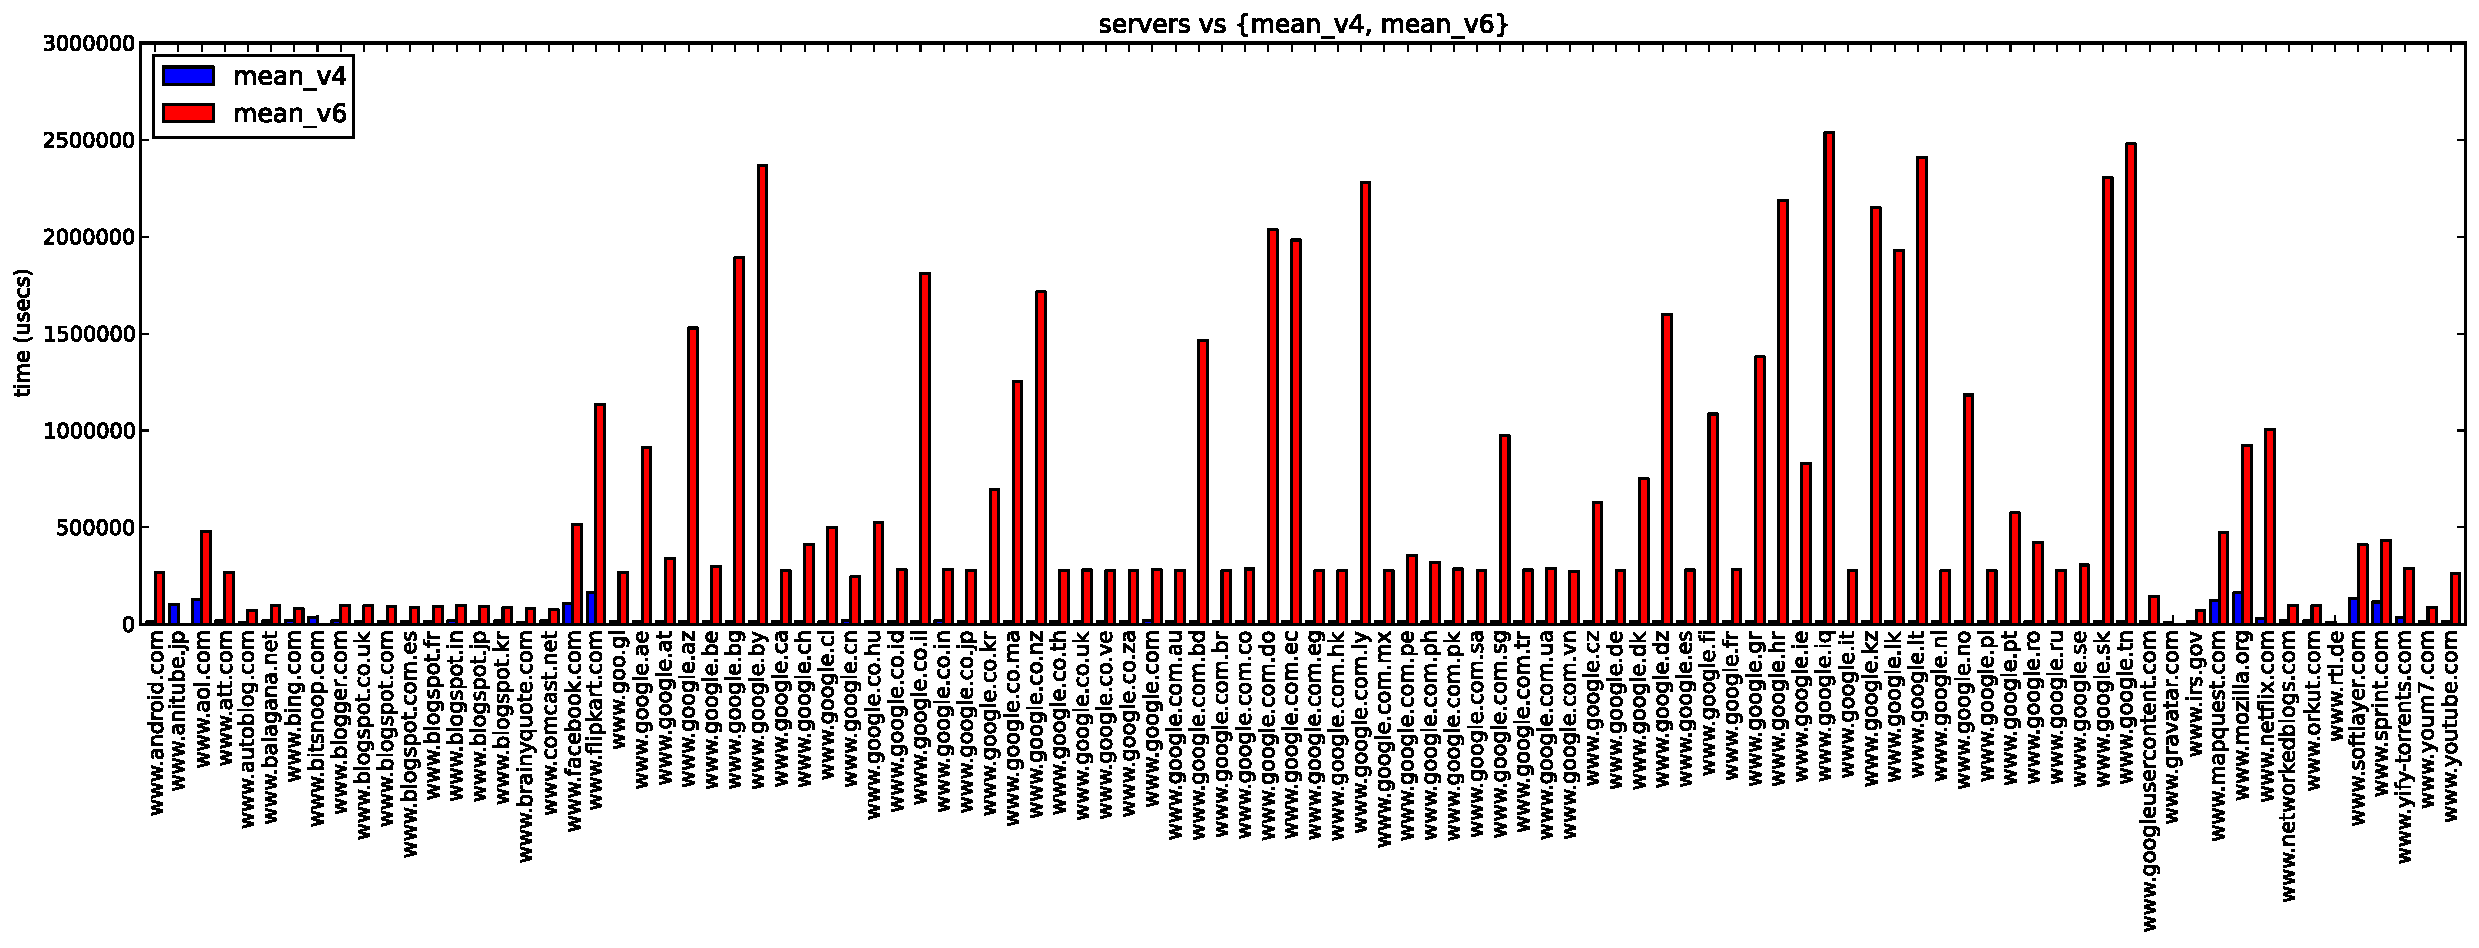
\includegraphics{figures/t28972-mean}}
    %\caption{Native IPv4 and Teredo Tunnel}
  %\end{minipage}
  %\begin{minipage}[t]{0.50\textwidth}
    %\centering
    %\resizebox*{1.0\textwidth}{!}{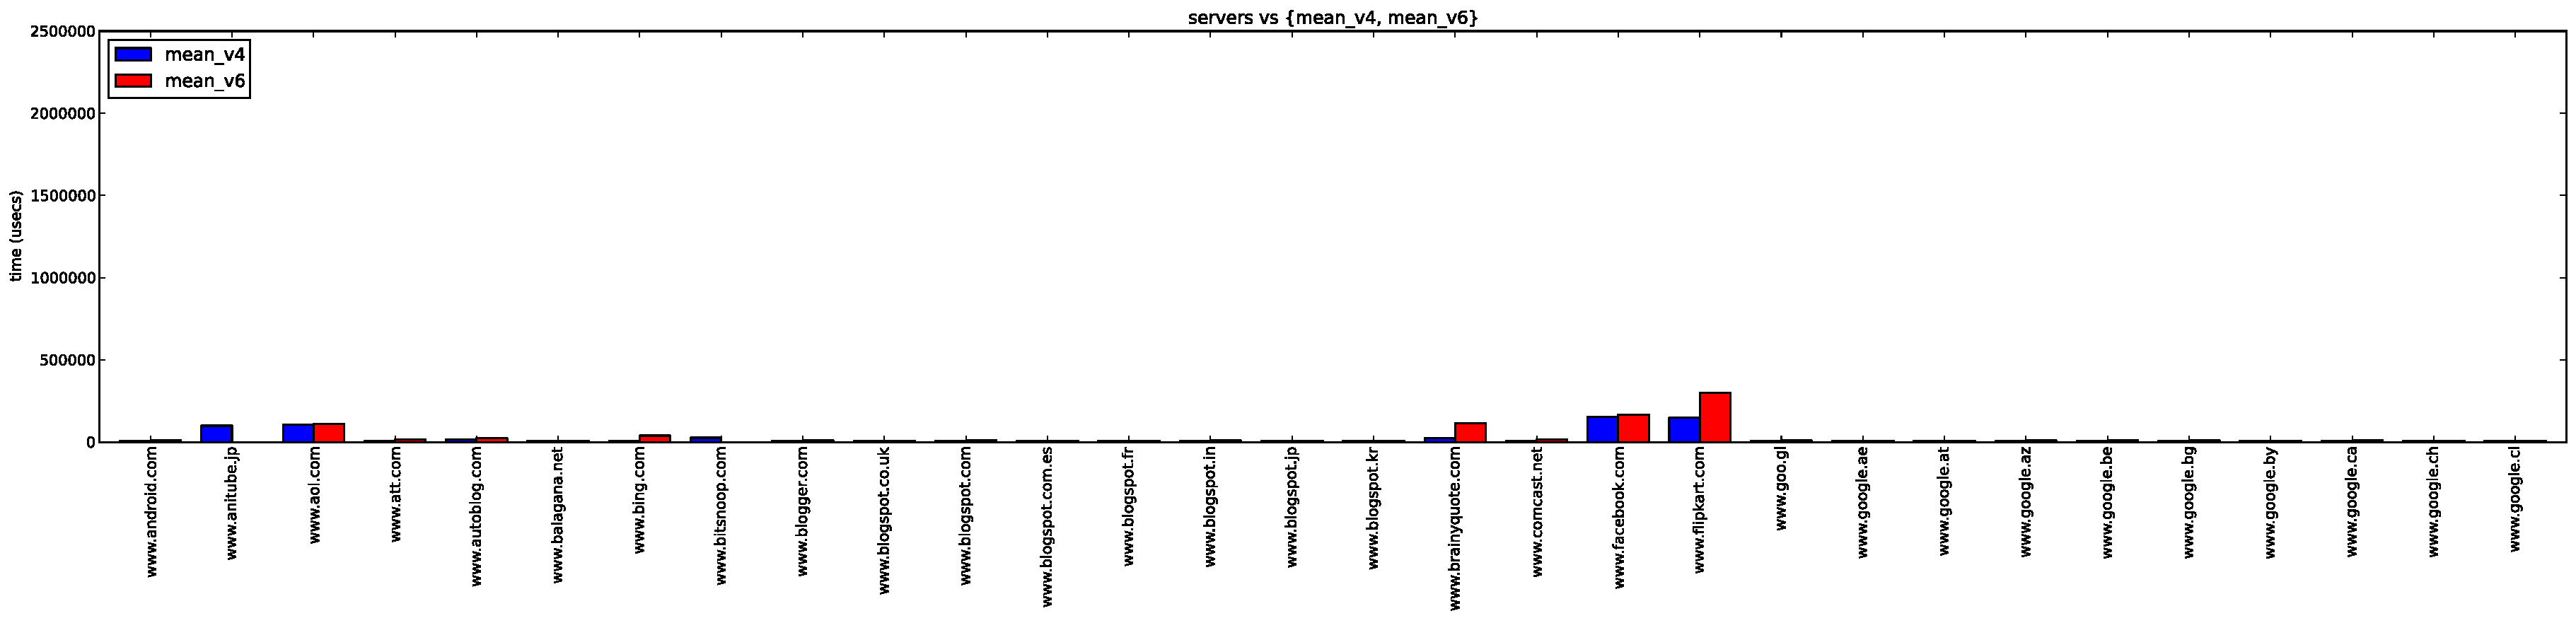
\includegraphics{figures/unimator2-mean}}
    %\caption{Native IPv4 and Native IPv6}
  %\end{minipage}
%\caption{\label{fig:happy-v4-v6-mean-std} Mean and Standard Deviations for
%IPv4 and IPv6}
%\end{figure}

This noticeable degraded user experience can be subverted by making
applications apply the happy eyeballs algorithm \cite{rfc6555}. The algorithm
recommends that an end-host after resolving the DNS name of a dual-stacked
service, tries a TCP \texttt{connect(\ldots)} to the first endpoint (usually
IPv6). However, instead of waiting for a timeout, it only waits for 300ms,
after which it must initiate another TCP \texttt{connect(\ldots)} with a
second address family and start a competition to pick the one that completes
first.  In this pursuit, to determine whether applications will use IPv4 or
IPv6 on a dual stacked service, we developed \texttt{happy}, a simple TCP
happy eyeballs probing tool. It uses non-blocking \texttt{connect(\ldots)}
calls to concurrently establish connections to all the endpoints of a service.
We have cross-compiled \texttt{happy} for the OpenWRT platform, so that the
tool can now be run on widely deployed SamKnows probes. In order to ascertain
the value in this approach, and develop data-analysis tools, we have prepared
an internal test-bed of multiple measurement points. The measurement points
have different flavors of IPv4 and IPv6 connectivity ranging from native IPv4,
native IPv6, IPv6 tunnel broker endpoints, Teredo and tunnelled IPv4. We used
the top 100 DNS names compiled by
\texttt{he.net}\footnote{\url{http://bgp.he.net/ipv6-progress-report.cgi}} and
ran \texttt{happy} on them.

\begin{figure}[t]
  \begin{minipage}[t]{0.50\textwidth}
    \centering
    \resizebox*{1.0\textwidth}{!}{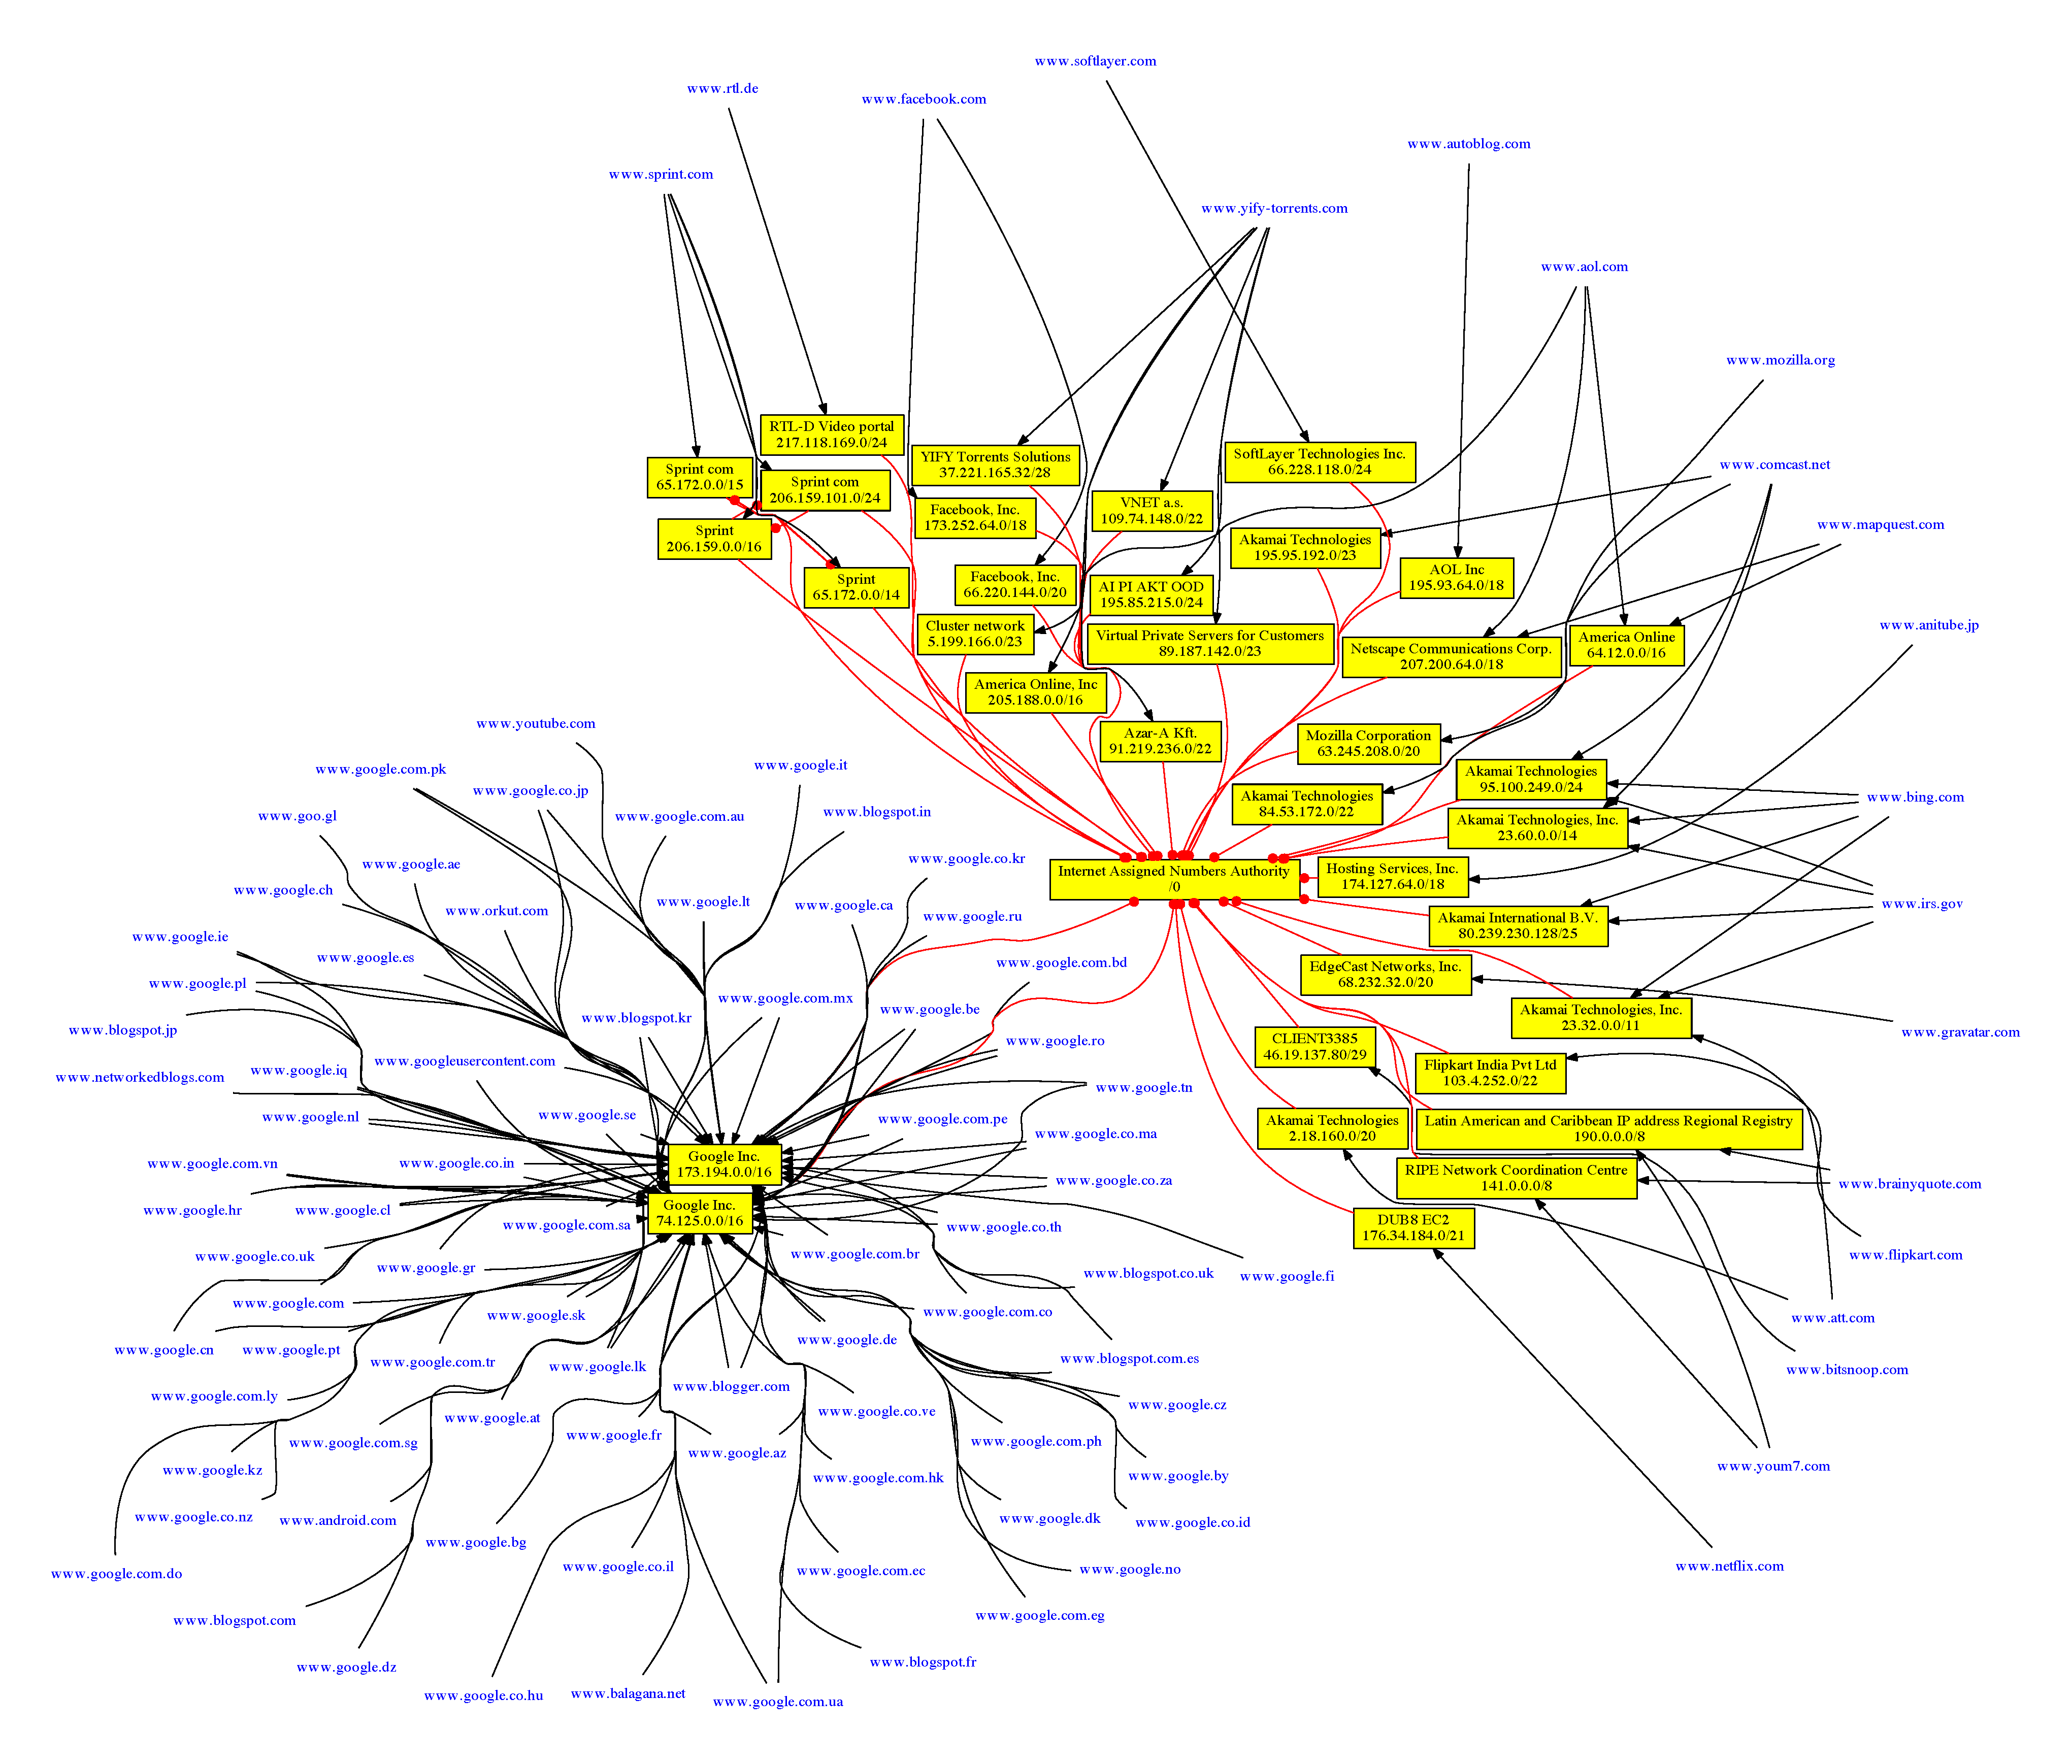
\includegraphics{figures/happy-v4cloud}}
  \end{minipage}
  \begin{minipage}[t]{0.50\textwidth}
    \centering
    \resizebox*{1.0\textwidth}{!}{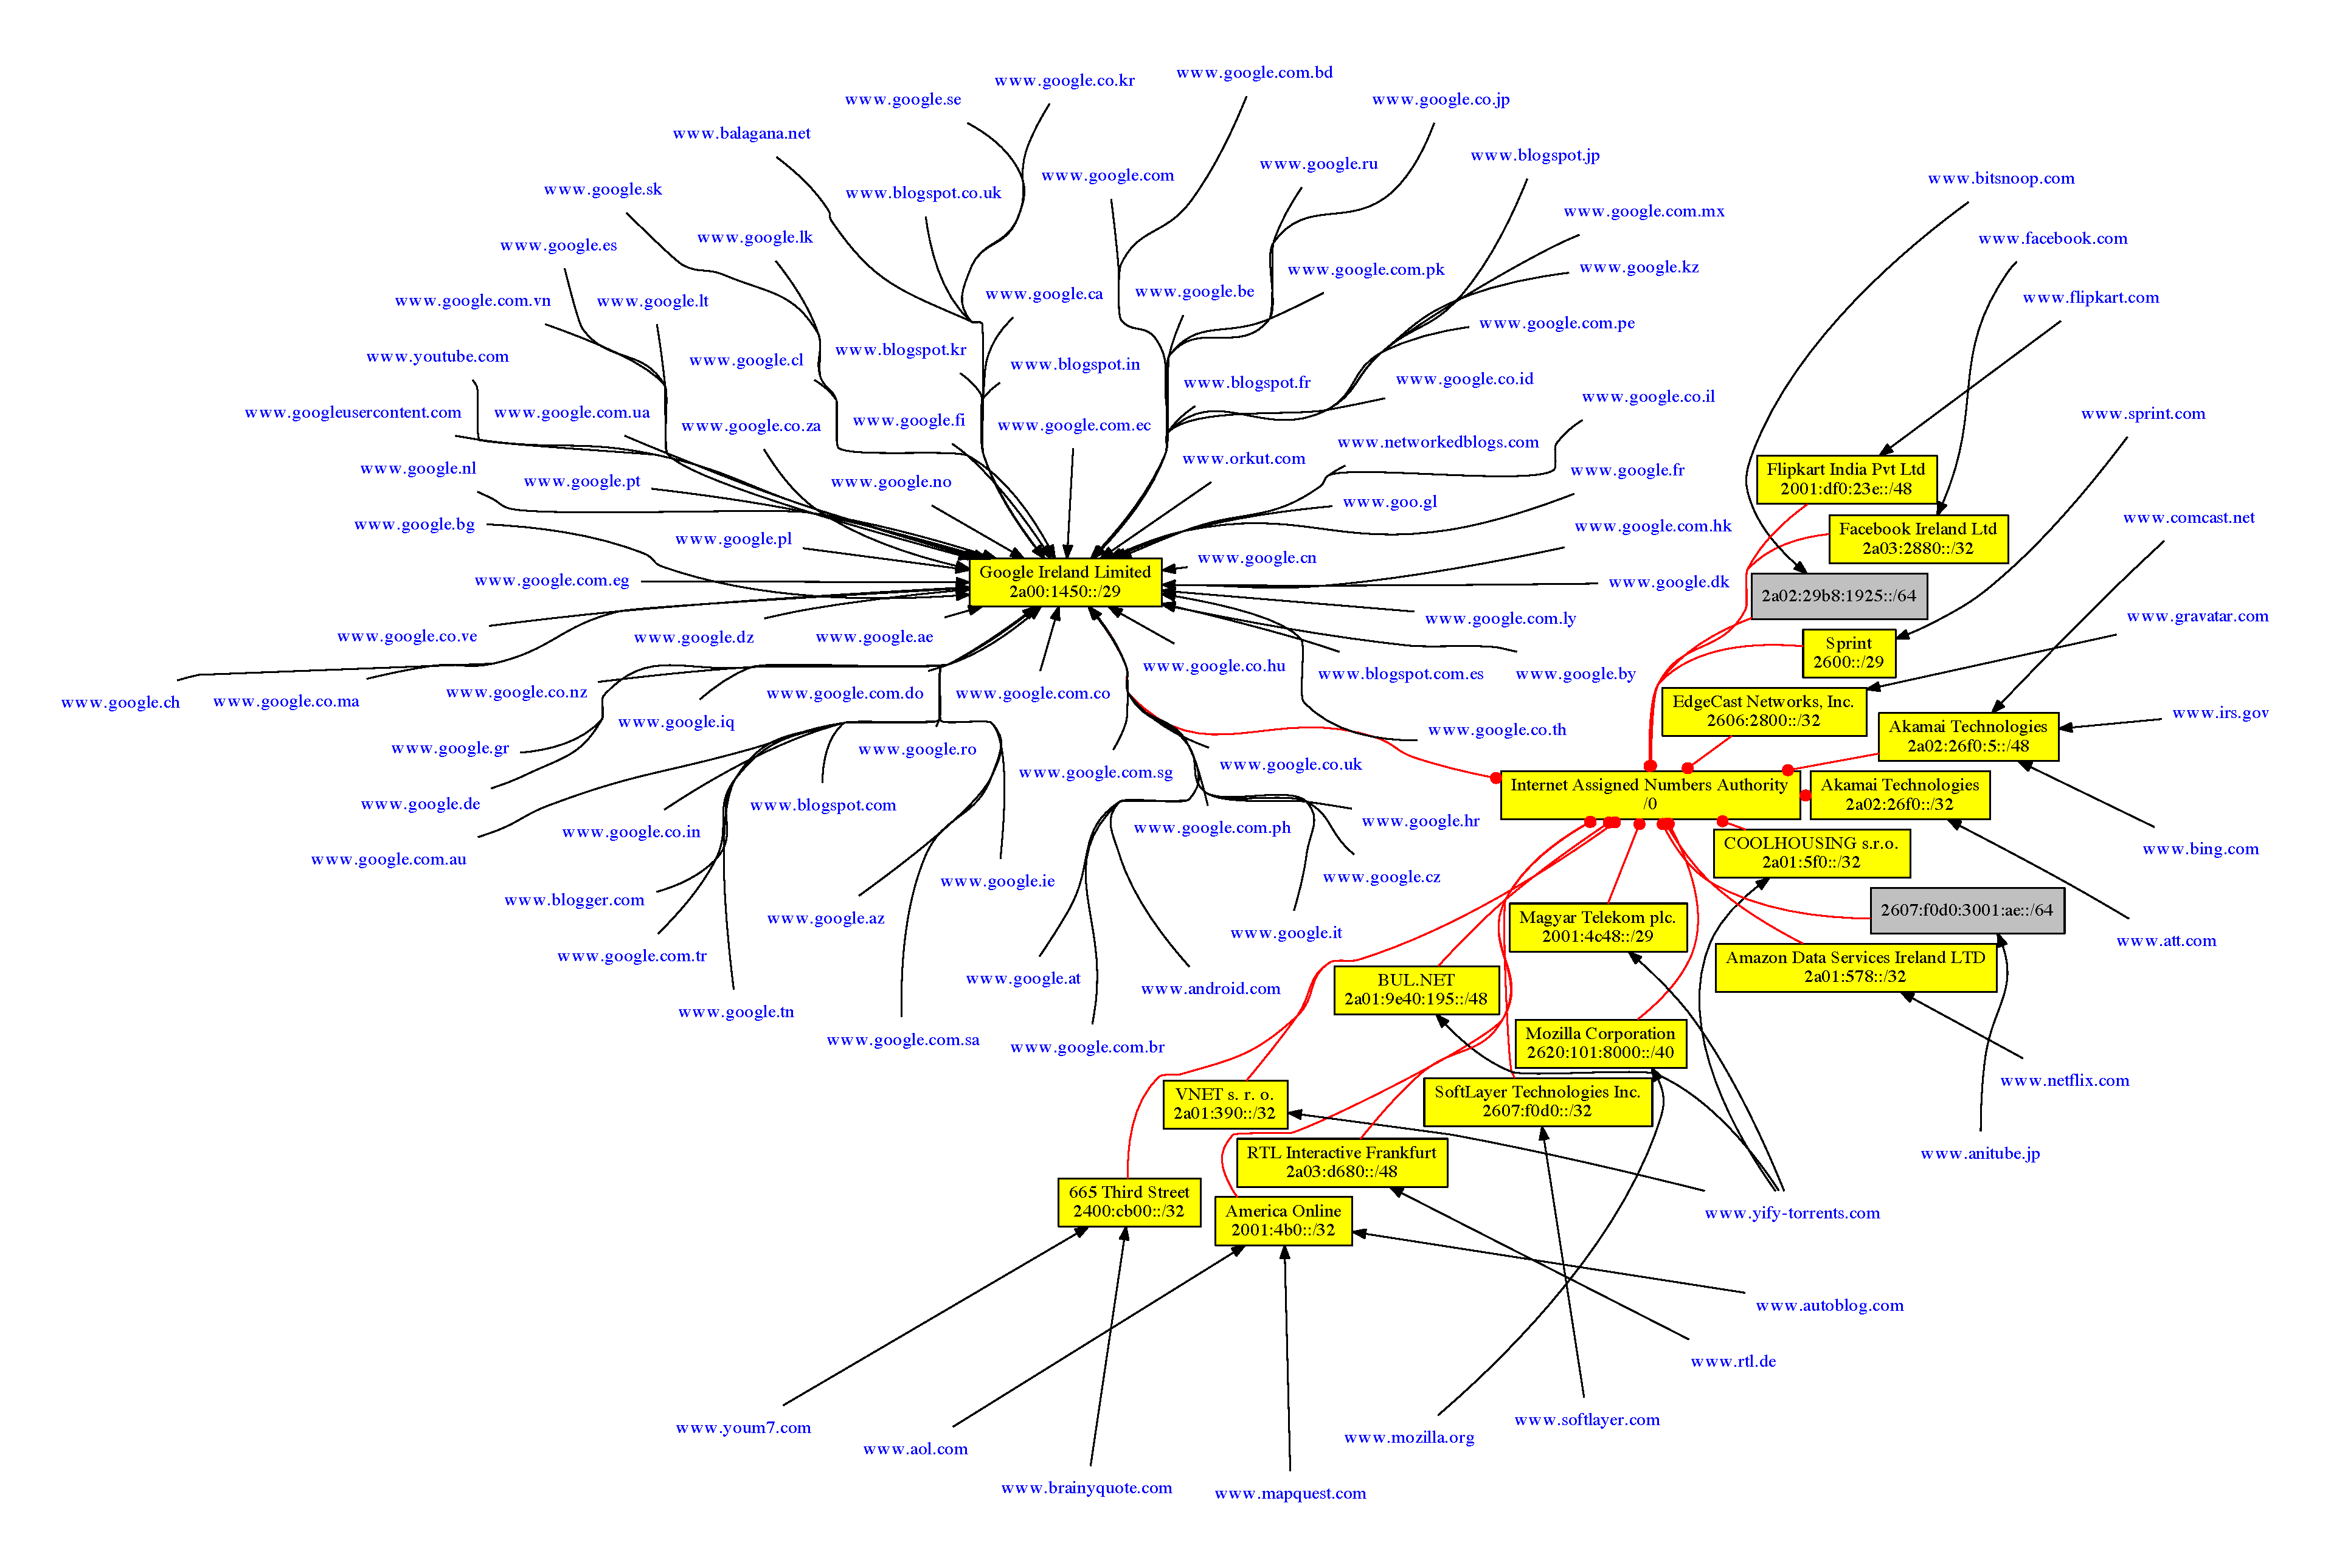
\includegraphics{figures/happy-v6cloud}}
  \end{minipage}
  \caption{\label{fig:v4-v6-cloud}An IPv4 and IPv6 aggregation cloud depicting
how most of the services centralize on core content delivery networks and
major cloud platforms (A full resolution image is available at
\texttt{https://gist.github.com/vbajpai/4730696})}
\end{figure}

%A preliminary result comparing the preference of a happy-eyeballed application
%to IPv6 and IPv4 from two measurement points is shown in Fig.
%\ref{fig:happy-v4-v6-compete}. The initial results show that happy eyeballs
%prevents IPv6 access to Facebook, with only a 20\% chance to get to Google
%related services over a Teredo Tunnel. The results look more promising on a
%native IPv6 connection. It is important to note that adhering to the happy
%eyeballs recommendation, IPv6 endpoints are allowed a 300ms chance to succeed.

A preliminary result comparing the mean time to establish a TCP connection to
each of the services from the one of the measurement points is shown in Fig.
\ref{fig:t28972-mean}. The initial results show higher connection times over
IPv6. We also noticed that given an option, there is a high probability, that
a happy eyeballs application will prefer IPv4 over Teredo IPv6. As such,
Teredo IPv6 will only be used when IPv4 connectivity is broken. In addition,
it appears, some of the related (and few of the unrelated) services show very
similar performances.  These services either resolve to the same endpoint or a
set of endpoints that belong to the same allocated prefix.  Digging through
the \texttt{whois} information for each of the endpoints from their \ac{RIR}
seems to indicate that major portion of the services map to allocated prefixes
owned by popular organizations like Google and Akamai Technologies as shown in
Fig.  \ref{fig:v4-v6-cloud}

%As much as it is important to define and implement new tests on these
%measurement infrastructure, it is also equally pertinent to not only be able
%to install, update and delete these tests but also configure the entire suite
%of probes using a standardized protocol over the network. The \ac{NETCONF}
%protocol \cite{rfc6241} is particularly designed to cater to this problem.
%Towards this end, we have built a \ac{NETCONF} server for the OpenWRT platform
%using the \texttt{libnetconf}
%\footnote{\url{http://code.google.com/p/libnetconf/}} library and tested the
%implementation using our NETCONF Python API \texttt{ncclient}
%\cite{sbhushan:2009}. This will allow automated deployment of measurement
%tests and remote management of their startup configurations.

